\documentclass{article}
\usepackage[utf8]{inputenc}
\usepackage{graphicx}
\usepackage{hyperref}
\graphicspath{ {images/} }
\usepackage[a4paper]{geometry}
\usepackage{minted}
\geometry{verbose,tmargin=2cm,bmargin=2cm,lmargin=2cm,rmargin=2cm}


\title{AIT - ZABBIX}
\author{Oplt Frantisek }



\usepackage{natbib}
\usepackage{graphicx}

\begin{document}



\maketitle
\newpage
\tableofcontents
\newpage
\section{Co je ZABBIX}
ZABBIX vytvořil Alexei Vladishev, a v současnosti je aktivně vyvíjen a podporován organizací ZABBIX SIA.je to nástroj monitorovací open source nástroj do firemního prostředí. ZABBIX umí monitorovat značné množství parametrů počítačové sítě a stav serverů.ZABBIX používá flexibilní oznamovací mechanismus, který umožňuje uživatelům konfigurovat e-mailové upozornění pro prakticky libovolnou událost.
\subsection{Co ZABBIX nabízí}
\subsubsection{Sběr dat}
    \begin{itemize}
        \item dostupnost a kontrola výkonu
        \item podpora SNMP, IPMI, JMX, monitorování VMware
        \item vlastní kontroly
        \item shromažďování požadovaných dat v obvyklích intervalech
    \end{itemize}
\subsubsection{Flexibilní definice prahových hodnot}
můžete definovat velmi flexibilní prahové hodnoty problému (triggers) odkazující na hodnoty z backendové databáze
\subsubsection{Vysoce konfigurovatelá oznámení}
odesílání oznámení lze přizpůsobit plánu eskalace, příjemce, typu média. Oznámení mohou být smysluplná a užitečná díky proměnným a makrům.
\subsubsection{Grafické zpracování v reálném čase}
sledované položky jsou okamžitě zaneseny do grafů pomocí vestavěné grafické funkce
\subsubsection{Možnosti webového sledování}
Zabbbix může sledovat cestu simulovaných kliknutí myší na webu a zkontrolovat funkčnost a dobu odezvy.
\subsubsection{Rozsáhlé možnosti vizualizace}
\begin{itemize}
    \item možnost vytvářet vlastní grafy, které mohou kombinovat více položek do jednoho zobrazení
    \item síťové mapy
    \item uživatelské obrazovky a prezentace pro přehled o dashboardové tabulce
    \item reporty
\end{itemize}
\subsubsection{Historické ukládání dat}
\begin{itemize}
    \item data jsou uložená v databázy
    \item konfigurovatelná historie
\end{itemize}
\subsubsection{Snadná konfigurace}
\begin{itemize}
    \item použití šablon
    \item použití šablon pro monitorování zařízení
\end{itemize}
\subsubsection{Prohlédání sítě}
\begin{itemize}
    \item automaticé zjišťování síťových zařízení
    \item automatická registrace agentů
    \item objevování souborových systémů, síťových rozhraní a SNMP OIDs
\end{itemize}
\subsubsection{Rychlé webové rozhraní}
\begin{itemize}
    \item webový frontend v PHP
    \item přístupné odkudkoliv
    \item ke všemu se dá proklikat
\end{itemize}
\subsubsection{Zabbix API}
Zabbix API poskytuje programovatelné rozhraní pro Zabix pro integraci do systému třetích stran
\subsubsection{Systém oprávnění}
\begin{itemize}
    \item zabezpečené ověření uživatele
    \item určití uživatelé mohou být omezeni na určité pohledy
\end{itemize}
\subsubsection{Agent}
Plně vybavený a snadno rozšiřitelný agent pro monitorování cílů, podporuje ajk Linux tak i Windows
\section{Zabbix procesy}
\subsection{Server}
Server je hlavním procesem programu Zabbix.
Server provádí dotazování a zachycování dat, vypočítá spouštěče (triggers)a odesílá oznámení uživatelům. Server je centrální repozidář, ve kterém jsou uložena všechna konfigurační, statistická a provozní data, a je to ta část Zabbixu, která bude aktivně upozorňovat správce na problémy, které nastanou v některem ze sledovaných systémů.
Funkce Zabbix serveru je rozdělena do tří odlišných komponent, jsou to:\newline
Zabbix server\newline
webový frontend\newline
databázový úložný prostor\newline
Všechny informace o konfiguraci pro službu Zabbix jsou uloženy v databázi, na které se soustředí server i webový frontend. Například při vytvoření nové položky pomocí webového frontend (nebo API) je přidán do tabulky položek v databázi. Pak asi jednou za minutu server Zabbix dotazuje tabulku položek na seznam aktivních položek, které jsou pak uloženy do vyrovnávací paměti v rámci serveru Zabbix. Proto může trvat až dvě minuty, než se všechny změny provedené v rozhraní Zabbix zobrazí v nejnovější části dat.
\subsubsection{Podporované platformy}

Kvůli bezpečnostním požadavkům a kritické povaze serveru je systém UNIX jediným operačním systémem, který může důsledně poskytovat pořebný výkon, toleranci k chybám a odolnost.
Server Zabbix funguje na těchto platformách:
\begin{itemize}
   \item Linux
   \item Solaris
   \item AIX
   \item HP-UX
   \item Mac OS X
   \item FreeBSD
   \item OpenBSD
   \item NetBSD
   \item SCO Open Server
   \item Tru64/OSF1
\end{itemize}
\subsection{Agent}
Agent Zabbix je nasazen na monitorovaný cíl a aktivně monitoruje místní zdroje a aplikace (pevné disky, paměť, statistiky procesů atd.
Agnet shromažďuje provozní informace místně a data odešla na Zabbix Server na další zpracování. Při selhání (například plný pevný disk nebo havárie) může Zabbix aktivně upozornit administrátory konkrétního počítače , který ohlásil selhání.
\subsubsection{Pasivní a aktivní kontroly}
Agenti Zabbix mohou provádět pasivní nebo aktivní kontroly.\newline
Při pasivní kontrole reaguje agent na požadavek na zaslání údajů ze Serveru. Server Zabbix (nebo proxy) požádá o data, například zatížení procesoru a agent Zabbix odešle výsledek zpět.\newline
Aktivní kontroly vyžadují složitější zpracování. Agent musí nejprve načíst seznam položek ze serveru Zabbix pro nezávislé zpracování. Poté bude periodicky odesílat nové hodnoty serveru.
Zda se provádí pasivní nebo aktivní kontroly, je konfigurováno výběrem příslušného typu monitorovací položky. Agent Zabbix zpracovává položky typu "Zabbix agent" nebo "Zabbix agent (active)".

\subsubsection{Podporované platformy}
\begin{itemize}
\item Linux
\item IBM AIX
\item FreeBSD
\item NetBSD
\item OpenBSD
\item HP-UX
\item Mac OS X
\item Solaris: 9, 10, 11
\item Windows: všechny verze desktopů a serverů od verze XP
\end{itemize}
\subsection{Proxy}
Proxy Zabbix je proces, který může shromažďovat data sledování z jednoho nebo více sledovaných zařízení a odeslat informace na server Zabbix (chová se jako Zabbix Server). Všechna shromážděná data jsou lokálně ukládána do paměti a pak jsou přenesena na server Zabbix, ke kterému patří proxy server.\newline
Nasazení serveru proxy je nepovinné, ale může být velmi výhodné pro zmenšení zátěže hlavního serveru Zabbix. Pokud se Zabbix server stará pouze o zpracování dat a ne o jejich zpracování (o to se postará proxy) tak server tolik nazatěžuje CPU a disk má méně I/O.\newline
Proxy Zabbix je ideálním řešením pro centralizované sledování vzdálených lokalit, poboček a sítí bez místních administrátorů.
\subsubsection{Podporované platformy}
Podporované platformy jsou stejné jako u serveru Zabbix
\subsection{Java gateway}

\subsection{Sender}
Zabbix sender je nástroj příkazového řádku, který může být použit k odeslání dat na server Zabbix pro zpracování.\newline
Nástroj je obvykle používán v dlouhých uživatelských skriptech pro periodické odesílání dat o dostupnosti a výkonu.
\subsection{Get}
Zabbix get je nástroj pro příkazovou řádku, který lze použít pro komunikaci s agentem Zabbix a získání požadovaných informací od agenta.\newline
Nástroj se obvykle používá k odstraňování problémů agentů Zabbix.
\section{instalace}
\subsection{získání zabbixu}
zabbix můžeme získat třemy způsoby.
\begin{itemize}
    \item instalce z distripučních balíčků
    \item stáhnout zdrojové kódy a sami si je zkompilovat
    \item stáhnout jako virtuální zařízení
\end{itemize}
\subsection{požadavky}
   Zabbix vyžaduje fyzickou i diskovou paměť. 128 MB fyzické paměti a 256 MB volného místa na disku by mohlo být dobrým výchozím bodem. Množství požadované paměti disku ovšem závisí na počtu monitorovaných hostitelů a parametrů. Pokud plánujete zachovat dlouhou historii sledovaných parametrů, měli byste přemýšlet alespoň o pár gigabajtů, abyste měli dostatek místa pro uložení historie do databáze. Každý proces démona Zabbix vyžaduje několik připojení k databázovému serveru. Množství paměti přidělené pro připojení závisí na konfiguraci databázového stroje.
\begin{center}
  \begin{tabular}{ | c | c | c | c | }
    \hline
    platforma & CPU/Memory & Databáze & Počet hostů \\ \hline
    CentOS & Virtual Appliance & MySQL InnoDB & 100 \\ \hline
    CentOS & 2 CPU cores/2GB & MySQL InnoDB & 500\\  \hline
    RedHat Enterprise Linux & 4 CPU cores/8GB & RAID10 MySQL InnoDB or PostgreSQL & >1000\\ \hline
    RedHat Enterprise Linux & 8 CPU cores/16GB & Fast RAID10 MySQL InnoDB or PostgreSQL & >10000\\  \hline
  \end{tabular}
\end{center}
\subsection{instalce pomocí balíčků - Debian/Ubuntu}
Zabbix balíky jsou k dispozici pro tyto verze:
\begin{itemize}
    \item Debian 9 (Stretch)
    \item Debian 8 (Jessie)
    \item Debian 7 (Wheezy)
    \item Ubuntu 16.04 (Xenial Xerus) LTS
    \item Ubuntu 14.04 (Trusty Tahr) LTS
\end{itemize}
Přidání repozitáře:
\begin{minted}{bash}
wget http://repo.zabbix.com/zabbix/3.4/ubuntu/pool/main/z/zabbix-release/zabbix-release_3.4-1+xenial_all.deb
echo dpkg -i zabbix-release_3.4-1+xenial_all.deb
sudo apt-get update
\end{minted}
\newline
instalace Zabbix serveru:
\begin{minted}{bash}
apt-get install zabbix-server-mysql
\end{minted}
\newline
instalace Zabbix proxy:
\begin{minted}{bash}
apt-get install zabbix-proxy-mysql
\end{minted}
\newline
instalce Zabbix frontendu:
\begin{minted}{bash}
apt-get install zabbix-frontend-php
\end{minted}
\newline
Pro správné fungování Zabbix server a Zabbix proxy se musí vytvořit databáze. (pro Zabbix agent není vyžadována)
\begin{minted}{bash}
shell> cd database/mysql
shell> mysql -uzabbix -p<password> zabbix < schema.sql
# stop here if you are creating database for Zabbix proxy
shell> mysql -uzabbix -p<password> zabbix < images.sql
shell> mysql -uzabbix -p<password> zabbix < data.sql
\end{minted}
Po vytvoření databáze do ní importujeme inicializační data
\begin{minted}{bash}
zcat /usr/share/doc/zabbix-server-mysql/create.sql.gz | mysql -uzabbix -p zabbix
# a pro proxy:
zcat /usr/share/doc/zabbix-proxy-mysql/schema.sql.gz | mysql -uzabbix -p zabbix
\end{minted}
Po importu dat upravíme soubory zabbix\_server.conf nebo zabbix\_proxy.conf a vložíme do nich údaje o databázi
\begin{minted}{bash}
# nano /etc/zabbix/zabbix_server.conf
DBHost=localhost
DBName=zabbix
DBUser=zabbix
DBPassword=<password>
\end{minted}
nakonec už stačí jenom zapnout službu zabbix
\begin{minted}{bash}
service zabbix-server start
\end{minted}
\subsection{instalace ze zdrojových souborů}
\subsubsection{stažení a rozbalení zdrojových kódů}
Ze stránek \url{www.zabbix.com} sis stáhneme archhiv se zdrojovími soubory. Jakmile máme archiv staený tak ho rozbalíme příkazem:
\begin{minted}{bash}
 tar -zxvf zabbix-3.4.0.tar.gz
\end{minted}
\subsubsection{vytvoření účtu}
Pro všechny procesy Zabbix je vyžadován uživatel bez oprávnění (normální uživatel). Pokud je démon Zabbix spuštěn z normálního účtu, poběží jako tento uživatel.
\newline
Ale pokud je démon zpoštěn z účtu "root", přepne se na uživatelský účet zabbix, který musí být přítomen. Vytvoření účtu:
\begin{minted}{bash}
 groupadd zabbix
 useradd -g zabbix zabbix
\end{minted}
\subsubsection{ vytvoření databáze}
Pro správné fungování Zabbix server a Zabbix proxy se musí vytvořit databáze. (pro Zabbix agent není vyžadována)
\begin{minted}{bash}
shell> cd database/mysql
shell> mysql -uzabbix -p<password> zabbix < schema.sql
# stop here if you are creating database for Zabbix proxy
shell> mysql -uzabbix -p<password> zabbix < images.sql
shell> mysql -uzabbix -p<password> zabbix < data.sql
\end{minted}
\subsubsection{konfigurace}
Když instalujeme Zabbix server nebo praxy ze zdrojových kódů, musíme specifikovat typ databáze.
\begin{minted}{bash}
# pro zobrazení všech možností konfigurace
./configure --help
# takto by nějak měla vypadat konfigurace
./configure --enable-server --enable-agent --with-mysql --enable-ipv6 --with-net-snmp --with-libcurl --with-libxml2
\end{minted}
\subsubsection{instalace}
Pro instalaci zabbixu stačí zadat příkaz "make install". Většinou je požadovánou použití uživatele root, nebo napsání příkazu "sudo".
\subsubsection{instalace webového rozhraní}
frontend zabbixu je napsán v PHP, takže pro jeho běh je požadován webový server s podporou PHP. Instalace je velmi jednoduchá, stačí překopírovat soubory z "frontend/php" to adresáře webového rerveru.
\newline
V prohlížeči zadáme adresu \url{http://<serverip_or_name/zabbix}
měla by se zobrazit následující obrazovka
\begin{center}
  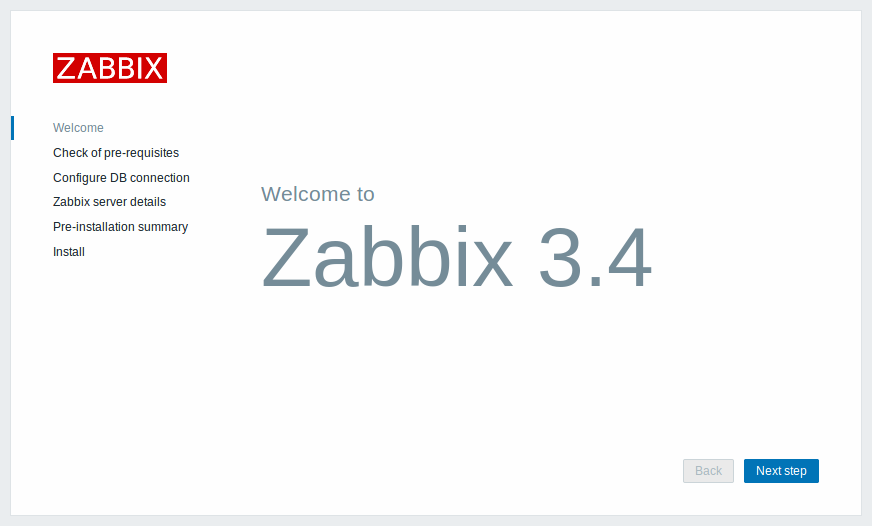
\includegraphics[width=0.7\textwidth]{obrazky/install_1.png}
\end{center}
Kontrola jestli systém splňuje minimální požadavky
\begin{center}
  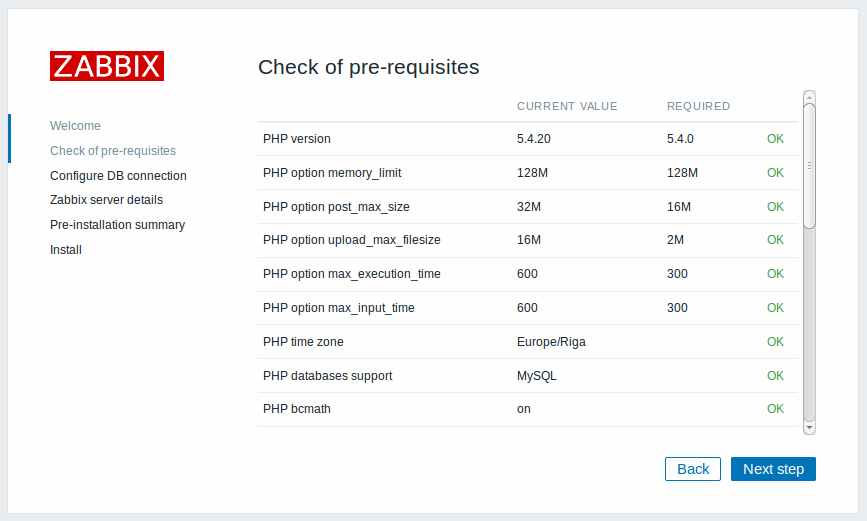
\includegraphics[width=0.7\textwidth]{obrazky/install_2.png}
\end{center}
vyplníme informace o databázi
\begin{center}
  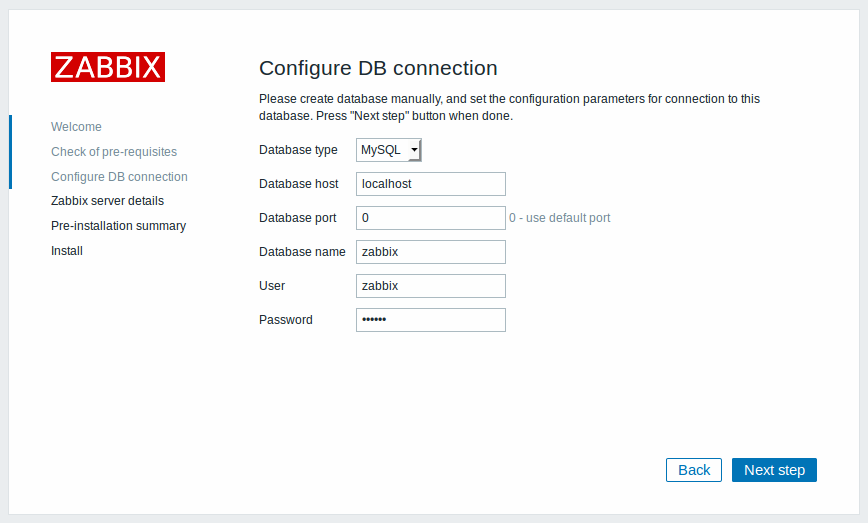
\includegraphics[width=0.7\textwidth]{obrazky/install_3.png}
\end{center}
doplníme informace o zabbixu
\begin{center}
  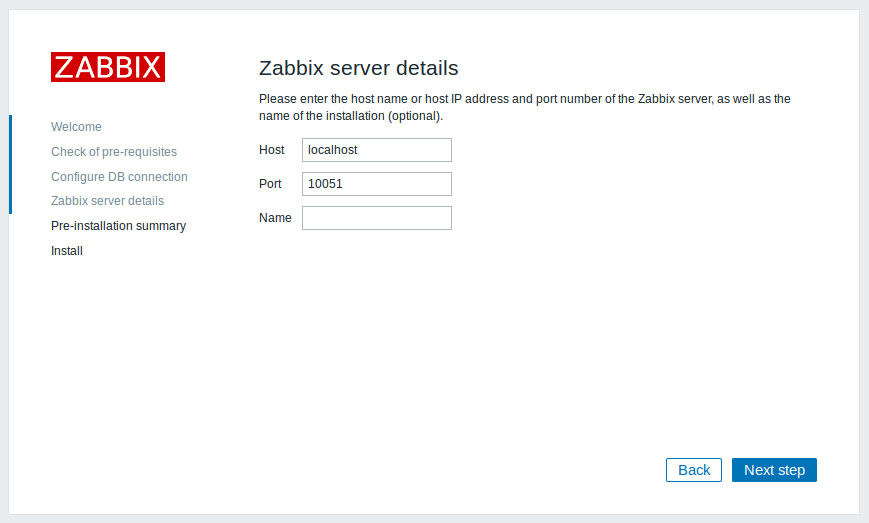
\includegraphics[width=0.7\textwidth]{obrazky/install_4.png}
\end{center}
shrnutí informací
\begin{center}
  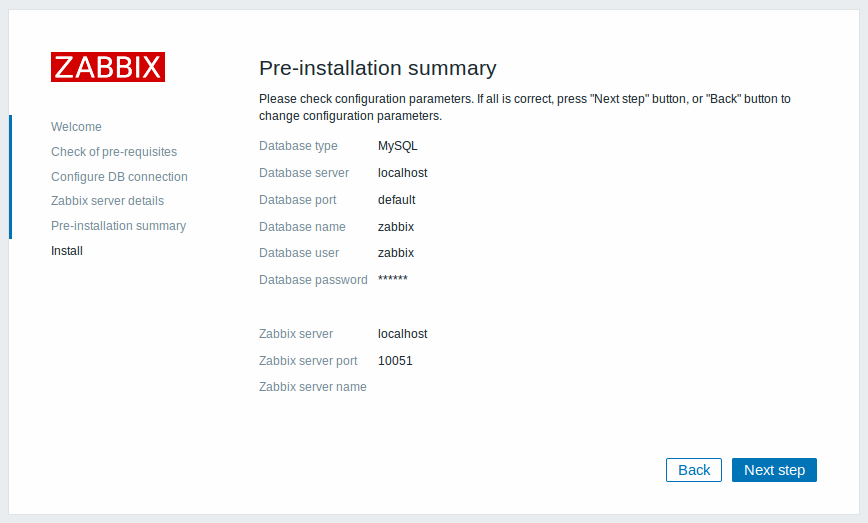
\includegraphics[width=0.7\textwidth]{obrazky/install_5.png}
\end{center}
musíme stáhnout konfikurační soubor na zkopírovat ho do složky conf/ na webovém serveru
\begin{center}
  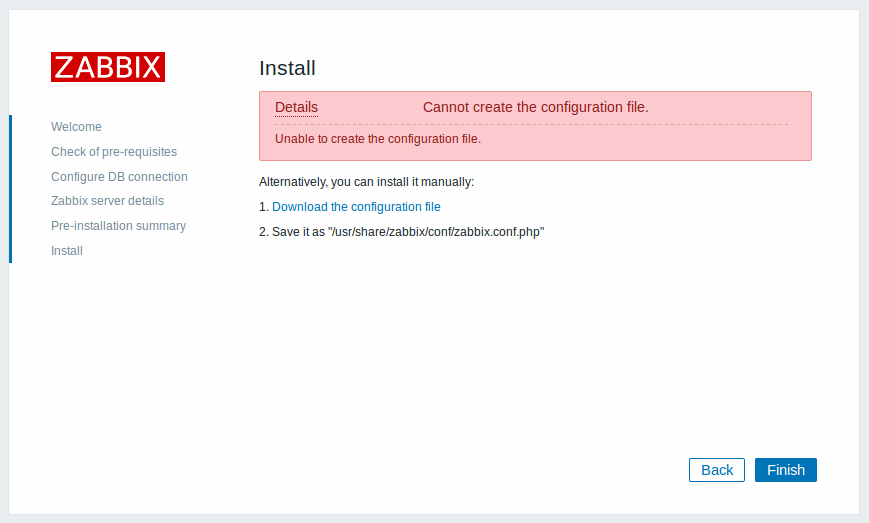
\includegraphics[width=0.7\textwidth]{obrazky/install_6.png}
\end{center}
\begin{center}
  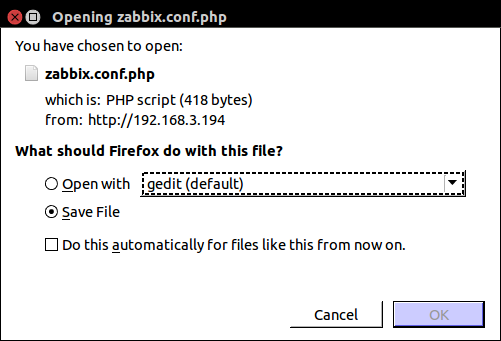
\includegraphics[width=0.7\textwidth]{obrazky/saving_zabbix_conf.png}
\end{center}
dokončení instalace
\begin{center}
  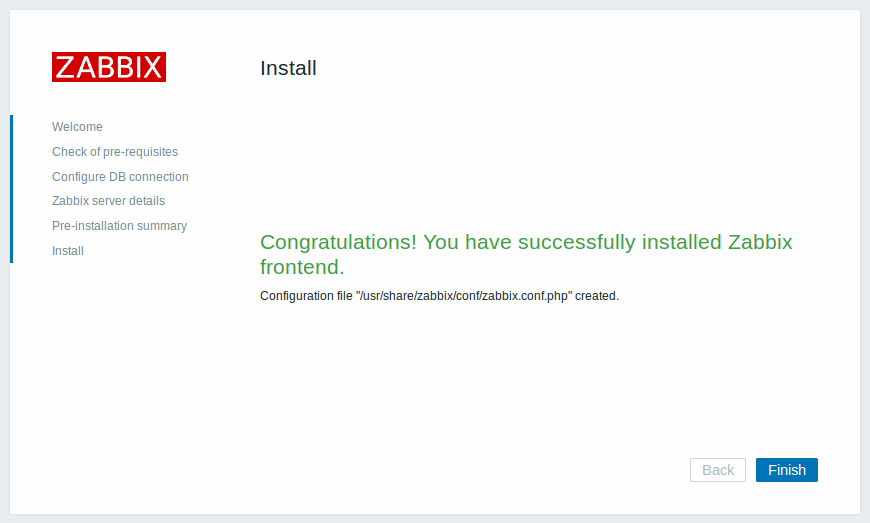
\includegraphics[width=0.7\textwidth]{obrazky/install_7.png}
\end{center}
niní už je zabbix připraven a stačí se přihlásit
\begin{center}
  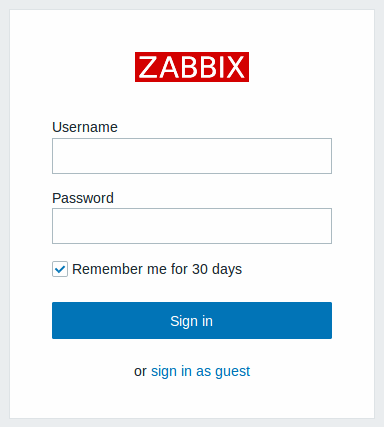
\includegraphics[width=0.7\textwidth]{obrazky/login.png}
\end{center}
\subsection{zabbix appliance}
jako aleternativu k ruční isntalaci můžeme stáhnout již připravený obraz operačního systému s předinstalovaným Zabbixem. Můžeme stáhnout jako iso nebo jako virtuální počítač.+ě 
\section{konfigurace}
\subsection{Hosté a skupiny hostů}
Tipycký hosté jsou zařízení, které si přejeme monitorovat (servery, procovní stanice, atd..) Vytvoření hostů je jedna z prvních věcí které budeme muset na zabbixu konfiguravat. Například, pokud chceme monitorovat nějaký parametru na serveru "X", musíme nejdřív mytvořit hosta nazvaného "Server X" a potom mu přiřadit parametry které chceme sledovat.
\newline
konfiguraci hostů najdeme v záložce "configutation -> Hosts"
\begin{center}
  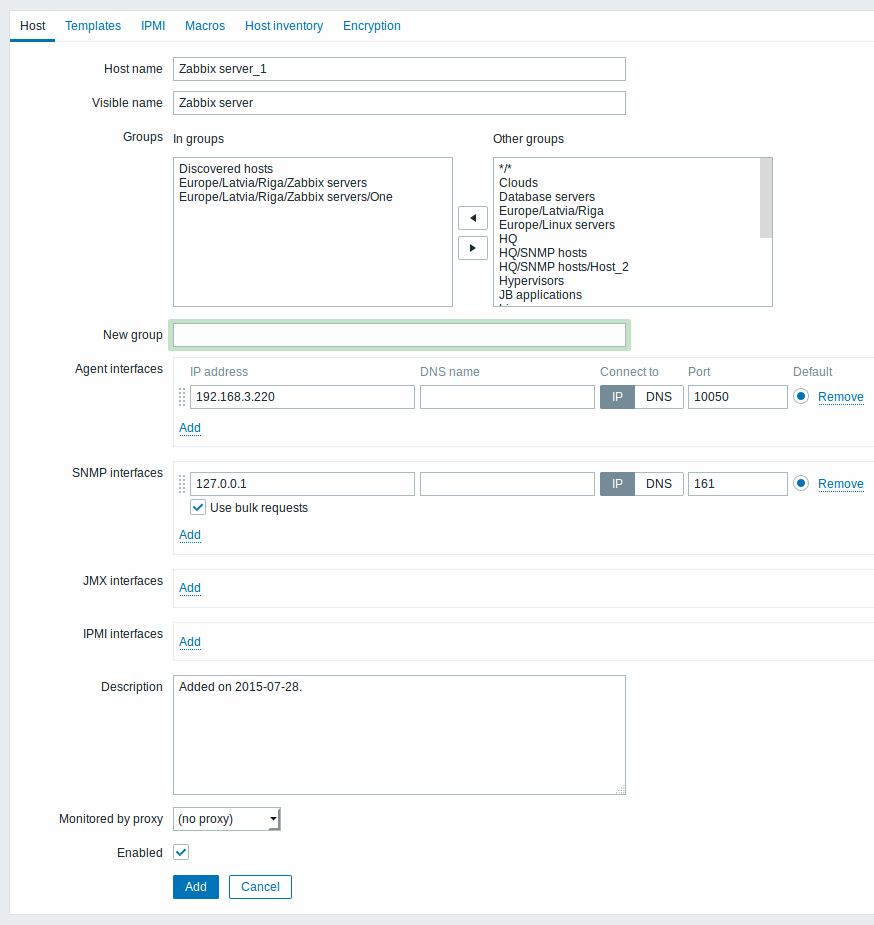
\includegraphics[width=0.7\textwidth]{obrazky/host_a.png}
\end{center}
\begin{center}
  \begin{tabular}{ | c | c | }
    \hline
    parametr & popis  \\ \hline
    Host name & unikátní jméno hosta \\ \hline
    Visible name & jméno které bude viditelné v seznamech, mapách, atd.\\  \hline
    Groups & Skupina do které host poatří \\ \hline
    New host group & vytvoření nové skupiny\\  \hline
    Interfaces & Zbůsob komunikace Hosta se Serverem (Agent, SNMP, JMX ... \\ \hline
    IP address & IP adresa hosta \\ \hline
    DNS name & DNS jméno hosta \\ \hline
    Connect to & tlačítko, kterým říkáme serveru jestli má použít IP adresu nebo DNS \\ \hline
    Port & TCP/UDP port přes, který komunikujeme s hostem \\ \hline
    Default & nastavení defaultních hodnot pro interface \\ \hline
    Description & Popis hosta\\ \hline
    Monitored by proxy & říkamá jestli chceme hosta monitorovat přes proxy server nebo příme ze Zabbix serveru \\ \hline
    Enabled & zaškrtnout jestli se má host monitorovat \\ \hline
  \end{tabular}
  \end{center}
  Záložka "Templates" vám umožní vybrat šablonu která se má použít na hosta. Veškeré parametry které sledujeme se odvýjí od zvoleného schématu.
  \subsection{Items (položky)}
   Items(položky) jsou schromážděná data z hosta. Jakmile je nakonfigurovaný host, je třeba přidat některé monitorovací položky, aby jsme mohli začít s získáváním aktuálních dat.
   \newline
   Jedním ze způsobů jak rychle přidat mnoho položek , je připojit k hostu jednu z předdefinovaných šablon. Pro optimalizaci výkonu systému je však dobré dolatit šablony tak aby obsahovali jen tolik položek, kolik je skutečně třeba. \newline
   K tomuto účelu použijete tlačítko "Items". Položka s názvem system.cpu.load tedy shromažďuje data o zatížení procesoru, zatímco položka s názvem net.if.in shromažďuje množství příchozí síťové komunikace.
   \newline
   Položka obsahuje následující parametry:
   \begin{center}
        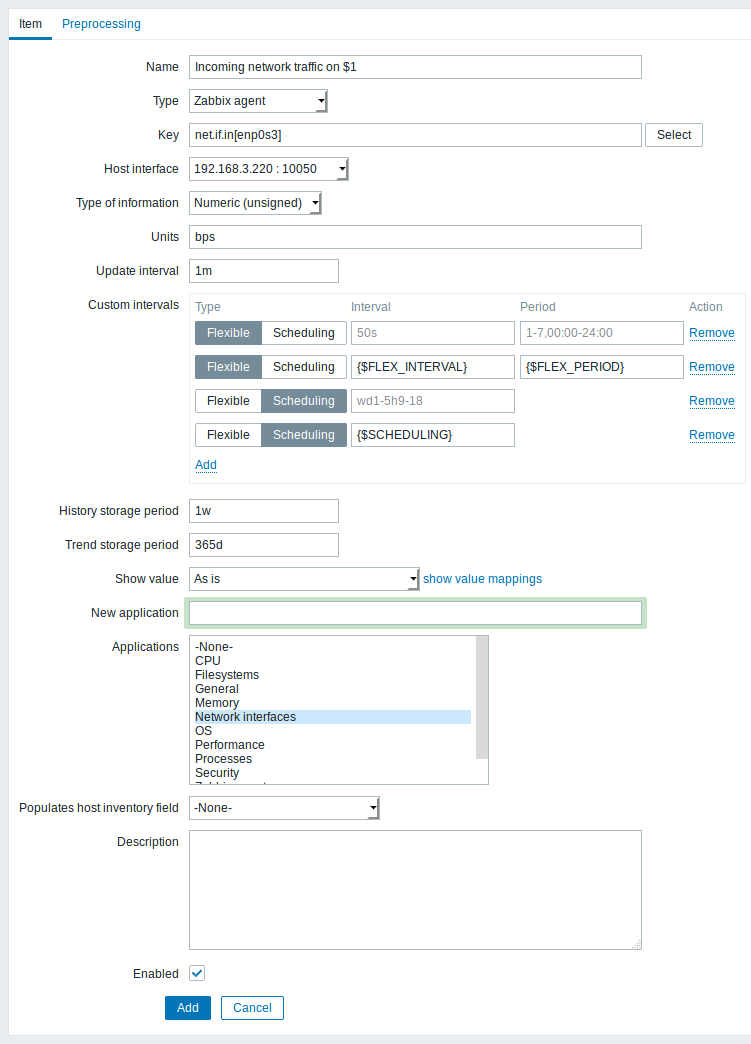
\includegraphics[width=0.7\textwidth]{obrazky/item.png}
   \end{center}
  
  \begin{tabular}{ | c | c | }
    \hline
    parametr & popis  \\ \hline
    name & jméno položky \\ \hline
    Type & typ položky\\  \hline
    Key & klíč. klíč musí být mít každá položka v hostovi unikátní \\ \hline
    Host interface & zvolit interface hosta\\  \hline
    Type of information & datov typ informace kterou chceme. Numeric, Character, Log, Text \\ \hline
    Units & jednotky, například Bps , Mps \\ \hline
    Update interval & Nová hodnota bude odeslána za N sekund \\ \hline
    Custom intervals & vlastní interval kdy budou chodit tada. Například každé pondělí od 8 do 12 \\ \hline
    History storage period & Jak dlouho bude uchovávána detailní historie v databázi (od 1 hodiny do 25 let)\\ \hline
    Trend storage period & Doba trvání uchování agregované (hodinové min, max, avg, počet) historie v databázi  \\ \hline
    Show value & mapování hodnot na tuto položku. Mapování hodnot nezmění přijaté hodnoty.
\\ \hline
    Log time format & dostupný jenom pro datový typ Log. \\ \hline
    New application & Zadejte název nové aplikace pro danou položku. \\ \hline
    Applications & odkaz položky na jednu nebo více stávajících aplikací. \\ \hline
    Populates host inventory field & Můžete vybrat pole inventáře hostitele, které bude obsahovat hodnotu položky. \\ \hline
   Description & popis položky \\ \hline
    Enabled & zaškrtnout jestli se má host monitorovat \\ \hline
  \end{tabular}
 \subsection{Triggers}
 Trigery jsou logické výrazy, které "vyhodnocují" data shromážděná podle položek a reprezentují aktuální stav systému.\newline
 Trigery umožňují definovat prahovou hodnotu toho, jaký stav dat je "přijatelný". Pokud příchozí data překročí přijatelný stav, spustí se trigger nebo změní stav na PROBLEM.
 \subsection{eventy}
V Zabbixu je generováno několik typů událostí:

trigger events -vždy, když spouštěč změní svůj stav  (OK→PROBLEM→OK)
\newline discovery events -  pokud jsou detekovány hosté nebo služby
auto registration events -  když jsou aktivní agenti automaticky registrováni serverem
\newline
Změna stavu trigeru je nejčastějším a nejdůležitějším zdrojem událostí. Pokaždé, když trigger změní svůj stav, generuje se událost. Událost obsahuje podrobnosti o změně stavu triggeru - kdy se to stalo a jaký je nový stav. 
\subsubsection{Prolem event}
    Problem event je vytvořený když:
    \begin{itemize}
        \item kdy je trigger výraz vyhodnocen TRUE, pokud je trigerr ve stavu OK
        \item pokaždé, když je trigger vyhodnocen TRUE, pokud je pro trigger povoleno generování více událostí.
    \end{itemize}
\subsubsection{OK Event}
    OK event uzavírá související problem event a může být spuštěn třemi komponentami:
    \begin{itemize}
        \item trriger
        \item korelace událostí
        \item task manager – event je ručně označen za ukončený
    \end{itemize}
\subsubsection{korelace událostí}
Korelace událostí je způsob, jak nastavit vlastní ukončení událostí (vygenerování OK události).\newline
\subsection{vizualizace}
\subsubsection{grafy}
S množstvím dat přicházející do Zabbixu je pro uživatele mnohem jednodušší, pokud se mohou podívat na vizuální reprezentaci dat.
Zabbix poskytuje uživatelům:
\begin{itemize}
        \item vestavěné jednoduché grafy dat jedné položky
        \item možnost vytvářet složitější přizpůsobené grafy
        \item přístup k porovnání několika položek rychle v ad-hoc grafech
    \end{itemize}
\subsubsection{Jednoduché grafy}
Pro vizualizaci dat shromážděných podle položek jsou k dispozici jednoduché grafy.\newline
Na uživatelské části není potřeba žádné konfigurační úsilí k zobrazení jednoduchých grafů. Jsou zdarma k dispozici firmou Zabbix.\newline
Jednoduše přejděte na Monitoring → Last data a klikněte na odkaz Graph pro příslušnou položku a zobrazí se graf.
\subsubsection{vlastní grafy}
Zatímco jednoduché grafy jsou dobré pro prohlížení dat jedné položky, nenabízejí konfigurační schopnosti.
\newline
Pokud tedy chcete změnit styl grafu nebo způsob zobrazení řádků nebo porovnávat několik položek, například příchozí a odchozí provoz v jednom grafu, potřebujete vlastní graf.
\newline
Pro konfiguraci vlastního grafu  jděte do "configuration - Hosts (nebo Templates). Potom klikneme na Graphs v obrazovce Graphs klikneme na Create graph a upravíme parametry grafu.
\begin{center}
        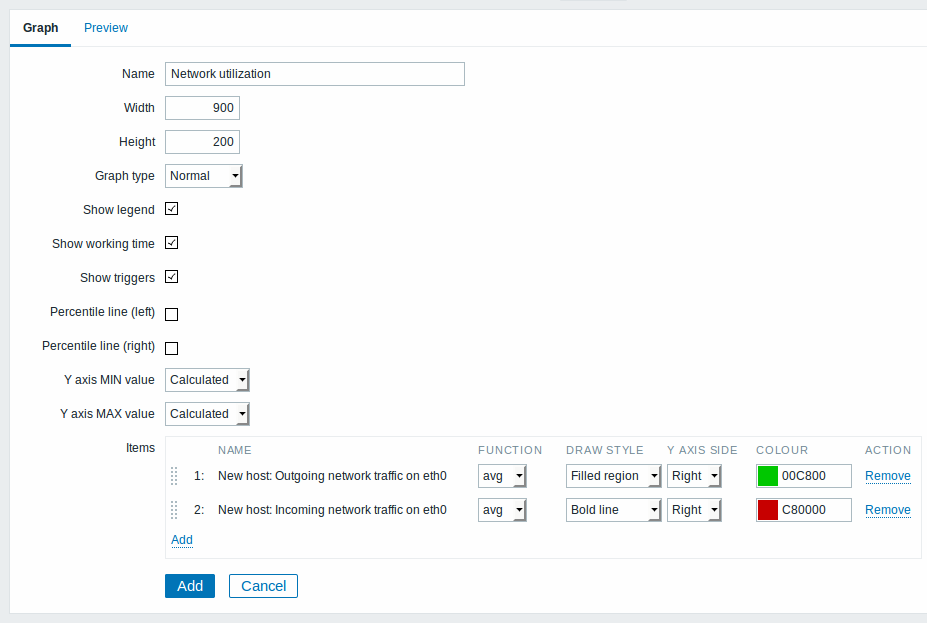
\includegraphics[width=0.7\textwidth]{obrazky/graph.png}
   \end{center}
\begin{itemize}
        \item Name -  název grafu
        \item Width - šířka grafu v pixelech
        \item Height - výška grafu v pixelech
        \item Graph type - typ grafu \begin{itemize}
            \item Normal - hodnoty jsou zobrazeny jako čáry
            \item Stacked - hodnoty jsou zobrazeny jko sloupce
            \item Pie - koláč
            \item Exploded - části koláče jsou vyříznuty ven
        \end{itemize}
        \item Show legend - zobrazit legendu ke grafu
        \item Show working time  - pokud je to zaškrtnuto tak ne-pracovní hodiny jsou v grafu zobrazeny šedě
        \item Show triggers - trigger bude zobrazen jako červená čára 
        \item Percentile line (left) - zobrazí procentuální čáru. například poku je 95\% tak udělá čáru pod kterou bude 95\% hodnot. Zobrazí se zeleně 
        \item Percentile line (right)  zobrazí procentuální čáru. například poku je 95\% tak udělá čáru pod kterou bude 95\% hodnot. Zobrazí se červeně 
        \item Y axis MIN value - Minimální hodnota na ose y (vypočítaná, fixní)
        \item Y axis MAX value - Maximální hodnota na ose y (vypočítaná, fixní)
        \item 3D view - zobrazí graf ve 3D
        \item Items - data která jsou zobrazen v grafu
    \end{itemize}
    \subsection{Ad-hoc grafy}
    Zatímco jednoduchý graf je skvělý pro přístup k datům jedné položky a vlastní grafy nabízejí možnosti přizpůsobení, žádný z nich neumožňuje rychle vytvořit srovnávací graf pro více položek s malým úsilím a žádnou údržbou.\newline
    od Zabbixu verze 2.4 toho lze dosáhnout pomocí ad-hoc grafu
    pro vytvoření ad-hoc grafu jdě do "Monitoring - Latest dat" použijte filtr pro zobrazení dat která chcete.  zaškrtněte které položky chcete zobrazit v grafu a klikněte na tlačítko Zobrazit zobrazené grafy nebo Zobrazit grafy.
    \begin{center}
        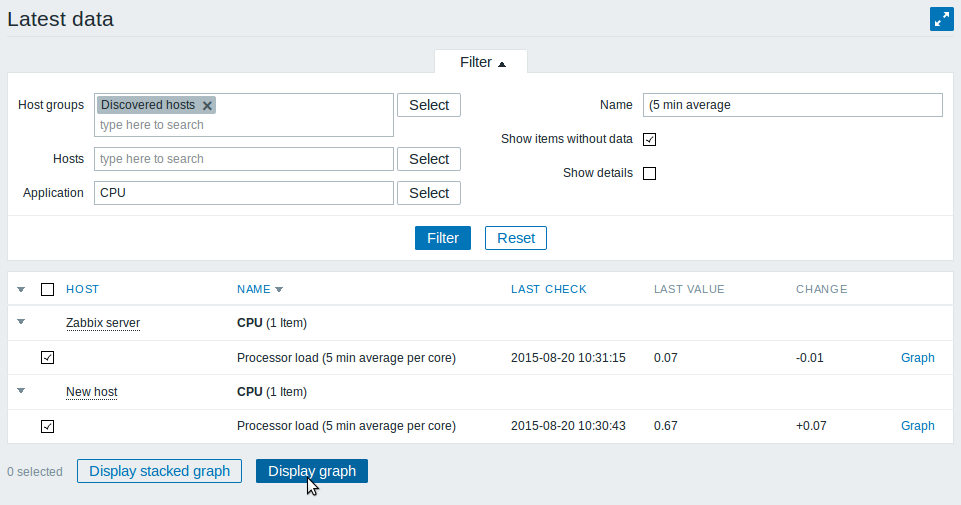
\includegraphics[width=0.7\textwidth]{obrazky/ad_hoc_graphs.png}
   \end{center}
  \subsection{Mapy sítí}
  Pokud máte síť, o kterou se chcete starat, možná budete chtít mít přehled o vaší infrastruktuře. Za tímto účelem můžete vytvářet mapy sítí v Zabbix.
  \newline
  Konfigurace mapy v Zabbixu vyžaduje, abyste nejprve vytvořili mapu definováním jejích obecných parametrů (rozměry, vlastník, ...) a poté začnete plnit mapu prvky a jejich odkazy.
  \newline
  Mapu vytvořime tak, že půjdeme do "monitoring - maps" klikneme na zobrazit všechny mapy a klikneme na "Create map"
  \begin{center}
        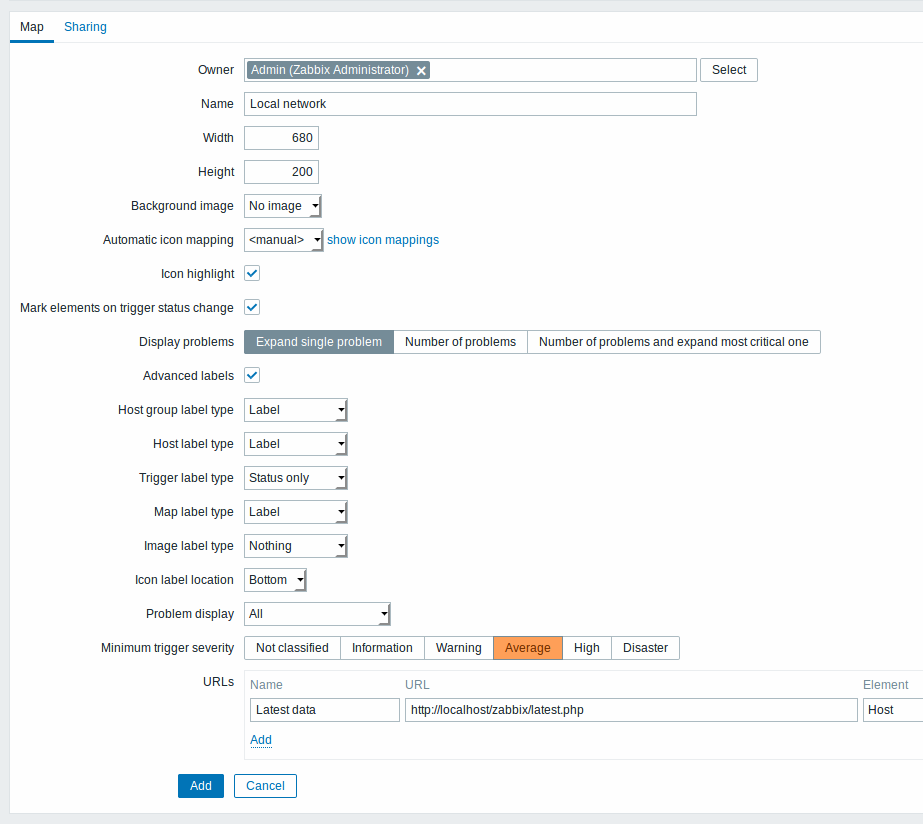
\includegraphics[width=0.7\textwidth]{obrazky/map_config.png}
\end{center}
\begin{itemize}
        \item Owner -  jméno vlastníka mapy
        \item Name - název mapy
        \item Width - sířka mapy
        \item Height - výška mapy
        \item Background image - pozadí
        \item Automatic icon mapping  - automatické mapování icon
        \item Icon highlighting - pokud je zařízení bez problému bude jeho icona obklopena zelenou čárou
        \item Mark elements on trigger status change - nedávné změny stavu triggeru budu na mapě zvýrazněny
        \item Display problems - na mapě budou zobraze pokud má nějaké zařízení problém
        \item Advanced labels - Zaškrtnutím tohoto políčka budete moci definovat samostatné typy štítků pro jednotlivé typy prvků.
        \item Icon label type - typ štítku používaný pro ikony \begin{itemize}
            \item Label - popisek ikony
            \item IP address - ip adresa
            \item Element name - název prvku (například název hosta)
            \item Status only - pouze status
            \item Nothing - žádný popisek nebude zobrazen
        \end{itemize}
        \item Icon label location - pozice popsiku
        \begin{itemize}
            \item Bottom - pod ikonou 
            \item Left - na levo od ikony
            \item Right  - na pravo od ikony
            \item Top  - nad ikonou
        \end{itemize}
        \item Problem display - zobrazení problémů
        \begin{itemize}
            \item All  - všechny problémy 
            \item Separated  - nepotvrzené problémy budou zobrazeny samostatně
            \item Unacknowledged only  - pouze nepotvrzené problémy
        \end{itemize}
        \item Minimum trigger severity - nejmenší úroveň triggeru která se bude zobrazovat
        \item URLs - Adresy URL pro každý typ prvku lze definovat (s popisem). Zobrazí se jako odkaz, když uživatel klikne na prvek v režimu zobrazení mapy.
    \end{itemize}
\subsubsection{přidání prvku do mapy}
      Chcete-li přidat prvek, klikněte na tlačítko Add vedle ikony. Nový prvek se objeví v levém horním rohu mapy. Přetáhněte ho tam, kam se chcete.
\subsection{Obrazovky}
Na obrazovkách Zabbix můžete seskupit informace z různých zdrojů a získat tak rychlý přehled o jedné obrazovce. Vytváření obrazovek je poměrně snadné a intuitivní.\newline
V podstatě je obrazovka tabulkou. Vybíráte, kolik buněk na tabulku a jaké prvky chcete zobrazit v buňkách. Mohou být zobrazeny následující prvky:
\begin{itemize}
    \item jednoduché grafy
    \item jednoduché grafické prototypy
    \item uživatelsky definované vlastní grafy
    \item vlastní grafické prototypy
    \item mapy
    \item další obrazovky
    \item prostý textu
    \item informace o serveru (přehled)
    \item informace o hostu (přehled)
    \item informace o triggeru (přehled)
    \item problémy hosta / skupiny hostů
    \item stav systému
    \item přehled dat
    \item hodiny
    \item historie událostí
    \item historie nedávných akcí
    \item Adresa URL (data z jiného místa)
\end{itemize}
Obrazovky jsou spravovány v části Monitoring → Screens, kde je lze konfigurovat, spravovat a prohlížet. \newline
Chcete-li nakonfigurovat obrazovku, musíte ji nejprve vytvořit tak, že definujete její obecné vlastnosti a potom do buněk přidáte jednotlivé prvky.\newline
Všichni uživatelé v Zabbixu (včetně uživatelů bez práv administrátora) mohou vytvářet obrazovky. Obrazovky mají vlastníka - uživatele, který je vytvořil.\newline
Obrazovky mohou být zveřejněny nebo soukromé. Veřejné obrazovky jsou viditelné pro všechny uživatele\newline
\subsection{Prezentace obrazovek}
V prezentaci můžete nakonfigurovat, že se v nastavených intervalech zobrazí několik obrazovek.

Někdy můžete chtít přepínat mezi některými nakonfigurovanými obrazovkami. Můžete mezi nimi přepínat ručně, dělat to více než jednou nebo dvakrát může být velmi nudné. Proto nám autoři Zabbixu připravili funkci prezentace.

Všichni uživatelé v Zabbixu (včetně uživatelů bez práv administrátora) mohou vytvářet prezentace. Prezentace mají majitele - uživatele, který je vytvořil.

Prezentace mohou být veřejné nebo soukromé. Veřejné prezentace jsou viditelné všem uživatelům, ale musí mít alespoň oprávnění ke čtení všech prvků (obrazovky) prezentace, aby je viděli. Chcete-li do prezentace přidat obrazovku, musí mít uživatel alespoň oprávnění ke čtení.
\section{Monitorování služeb}
Funkce monitorování služeb je určena pro ty, kteří chtějí získat vysoký (obchodní) pohled na monitorovanou infrastrukturu. V mnoha případech se nejedná o detaily na nízké úrovni, jako je nedostatek místa na disku, vysoká zátěž procesoru atd. To, co nás zajímá, je dostupnost služeb poskytovaných naším oddělením IT. Můžeme se také zajímat o identifikaci slabých míst IT infrastruktury, SLA různých IT služeb, struktury stávající IT infrastruktury a dalších informací vyšší úrovně.
\subsection{Konfigurace}
konfiguraci pro nastavení monitorování služeb najdeme v záložce "Configuration -> Služby"
Na této obrazovce můžete vytvořit hierarchii sledované infrastruktury. Rodičovská služba nejvyšší úrovně je "root". Hierarchii můžete vytvořit směrem dolů přidáním nižších úrovní rodičovských služeb a poté k jednotlivým uzlům
\begin{center}
        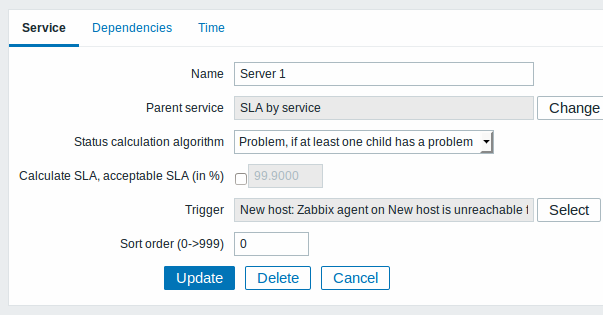
\includegraphics[width=0.7\textwidth]{obrazky/itservice.png}
\end{center}
Klepnutím na tlačítko "add child" přidáte službu. Chcete-li upravit existující službu, klikněte na její název. Zobrazí se formulář, kde můžete upravit atributy služby.
\begin{center}
        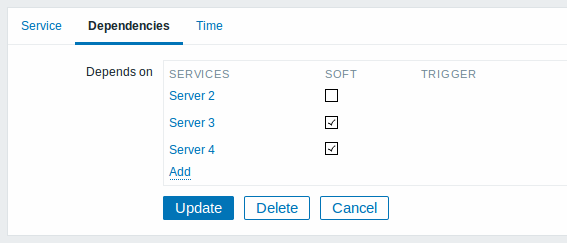
\includegraphics[width=0.7\textwidth]{obrazky/itservice_b.png}
\end{center}
Parametry: 
\begin{itemize}
    \item Name - Jméno služby
    \item Parent service - Nařazená služba pod kterou služba patří
    \item Status calculation algorithm - Metody pro kalkulaci statusu služby: \newline Do not calculate - nepočítá se stav služby
    \newline Problem, if at least one child has a problem  - problém pokud je alespoň jedna z podslužeb má problém
    \newline Problem, if all children have problems  - problém pokud májí všechny podslužby problém.
    \item Calculate SLA - Zapne SLA kalkulaci a zobrazí ji
    \item Acceptable SLA (in \%) - Procento SLA, které je pro tuto službu přijatelné. Používá se pro vytváření reportů.
    \item trigger - přiřazení k triggeu
    \newline None - žádné přiřazení
    \newline trigger name - název triggru
\end{itemize}
Pevná a měkká závislost
\newline
Dostupnost služby může záviset na několika dalších službách, nikoliv na pouze jedné. První možností je přidat všechny služby přímo jako podřízené služby.
\newline
Nicméně, pokud je některá služba již přidána někde jinde ve stromu služeb, nelze ji jednoduše přesunout z childe service. Jak vytvořit závislost? Odpověď je "měkká" závislost. Přidejte službu a zaškrtněte políčko Soft. Tímto způsobem služba může zůstat v původním umístění ve stromu, přesto však závisí na několika dalších službách. Služby, které jsou "soft-linked" jsou ve stromu zobrazeny šedě. Navíc, pokud má služba pouze "měkké" závislost, lze ji smazat přímo bez odstranění podřízených služeb.
\end{document}
